\section*{\large{ВВЕДЕНИЕ}}

Цель лабораторной работы --- разработать программу шифровальной машины <<AES>> \cite{Enigma}.

Задачи лабораторной работы:

\begin{enumerate}
    \item провести анализ работы шифровальной машина <<AES>>;
    \item описать алгоритм шифрования;
    \item релизовать описанный алгоритм.
\end{enumerate}

\clearpage
\section{Аналитическая часть}

\subsection{Алгоритм шифрования AES}

\textbf{AES} (Advanced Encryption Standard;) \cite{Enigma} --- симметричный алгоритм блочного шифрования (размер блока 128 бит, ключ 128/192/256 бит), принятый в качестве стандарта шифрования правительством США по результатам конкурса AES.

\textbf{Раунды шифрования}:

\begin{itemize}
	\item[---] \textbf{Деление на блоки}:в AES элементы организованы в матрицы 4 на 4 по 128 бит. Получается, нас есть сообщение размером 128 бит или 16 байтов в виде матрицы 4 на 4.
	\item[---] \textbf{Наложение фрагмента ключа через XOR}: Сначала функция SubBytes подставляет на место одних байтов другие из таблицы замены (S-блока). Затем ShiftRows сдвигает элементы в каждом ряду матрицы. После этого MixColumns перемешивает элементы в каждом столбце. Первый шаг – это подстановка, второй и третий – перестановка. В конце каждого раунда мы добавляем раундовый ключ (Round Key).
\end{itemize}

Алгоритм шифрования AES может использоваться в следующих режимах.

\begin{enumerate}
	\item[1.] \textbf{PCBC} (Cipher Block Chaining) --- режим сцепления блоков;
	\item[2.] \textbf{CBC} (Cipher Block Chaining) --- режим сцепления блоков;
	\item[3.] \textbf{CFB} (Cipher Feed Back) --- режим обратной связи по шифротексту;
	\item[4.] \textbf{OFB} (Output Feed Back) --- режим обратной связи по выходу.
\end{enumerate}

\clearpage

\section{Конструкторская часть}

\subsection{Разработка алгоритма}

На рисунке \ref{fig:algo} представлена схема алгоритма шифрования AES.

%

\begin{figure}[h!]
	\centering
	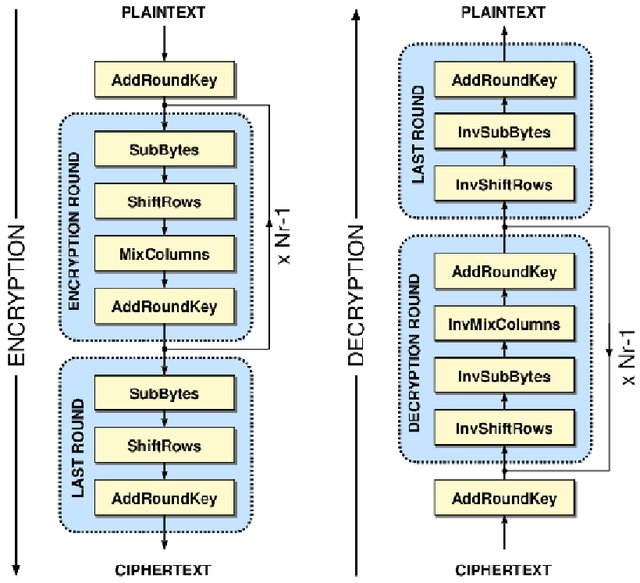
\includegraphics[width=\textwidth]{assets/images/AES.jpg}
	\caption{Схемы алгоритма AES}
	\label{fig:algo}
\end{figure}
\clearpage

\section{Технологическая часть}

\subsection{Средства реализации}

Для реализации ПО был выбран язык C++ \cite{c++}.
В данном языке есть все требующиеся инструменты для данной лабораторной работы.
В качестве среды разработки была выбрана среда VS code \cite{vscode}.

\subsection{Реализация алгоритма}

Реализация OFB.

\begin{lstlisting}
    void encrypt(FILE *inputData, FILE *outputData)
    {
        //input list of 16 bytes
        uchar list[16];
        int suffix=0;
        uchar temp=0x00;
        uchar *preC = IV;
        fwrite(preC,16,1,outputData);
        while(fread(list,16,1,inputData)==1)
        {
            unitEncrypt(list, preC);
            fwrite(list,16,1,outputData);
        }
    
        //encrypt least data, whose length < 128
        while((temp = fgetc(inputData)!=EOF))
        {
            list[suffix++] = temp;
        }
    
        if(suffix > 0)
        {
            for(int i=suffix; i<16; i++)
            {
                list[i] = 0x00;
            }
            unitEncrypt(list, preC);
            fwrite(list,16,1,outputData);
        }
    
        fclose(inputData);
        fclose(outputData);
    } 
\end{lstlisting}


\subsection{Тестовые данные}

В таблице \ref{tbl:functional_test} приведены тесты для алгоритма шифрования AES. 
Применена методология черного ящика. Тесты пройдены \textit{успешно}.



\begin{table}[ht!]
	\begin{center}
		\captionsetup{justification=raggedright,singlelinecheck=off}
		\caption{\label{tbl:functional_test} Функциональные тесты}
		\begin{tabular}{|c|c|c|}
			\hline
			Входная строка & Выходная строка \\ 
			\hline
			$ABOBA$ & $BCRGJ$\\
			$BCRGJ$  & $ABOBA$\\
			$<<>>$  & $<<>>$ \\
            $A$ & $T$\\
			$T$  & $A$\\
			\hline
		\end{tabular}
	\end{center}
\end{table}

\clearpage
\section*{\large{ЗАКЛЮЧЕНИЕ}}
В данной лабораторной работе:
\begin{enumerate}
    \item проведен анализ работы шифровальной машина <<AES>>;
    \item описан алгоритм шифрования;
    \item реализован описанный алгоритм;
\end{enumerate}